\section{Introduction}

In the even of an emergency, \acf{sUAS}


This chapter will extend offline landing site identification and selection methods described previously to support real-time operation using on-board sensors. Small UAS carrying LiDAR, RGBD cameras, or monocular cameras using Structure from Motion (SfM) can generate 3D point clouds of nearby landing sites. Polylidar3D can transform these dense point clouds to polygonal representations of flat-surfaces in real-time while accounting for obstacles.  Alternatively, many point cloud scans may be integrated into a larger cohesive mesh in which noise is reduced. The final mesh can then be sent to Polylidar3D for polygon extraction. In either case a previously-defined final touchdown site can be validated as obstacle-free or a new site defined as the largest inscribed circle within the polygon can be identified.
In the coming months, we propose to conduct a series of experiments in which a flying UAS hovers over obstacle-laden flat surfaces in the M-Air netted facility. Our landing site selection procedure can then be tested in real-time. M-Air offers a motion capture system to provide ground truth of the environment to allow accuracy assessment. Multiple LiDAR/camera combinations will be evaluated.

\paragraph{Preliminary Results}

In August 2019 the author (Castagno) interned at the NASA Langley Research Center to conduct experiments related to landing site selection. A custom built drone frame was used with an onboard Pixhawk flight controller, Intel NUC companion board, and a 16-beam Velodyne Puck Lite LiDAR. The LiDAR sensor was mounted at $45^{\circ}$ underneath the drone and flights were conducted in an indoor VICON-equipped motion capture facility as well as outside in a netted area with no motion capture. The basic setup for the experiments was to place obstacles in front of the drone, fly to an altitude above ground of 3.5m, and validate landing site selection algorithms. Figure \ref{fig:ch6_experiment} demonstrates one of the nine flight experiments conducted (six indoors and three outside). All data was captured and retained for later processing with possible algorithmic refinement.

\begin{figure}[ht]
    \centering
    \begin{subfigure}[t]{0.45\linewidth}
        \centering
        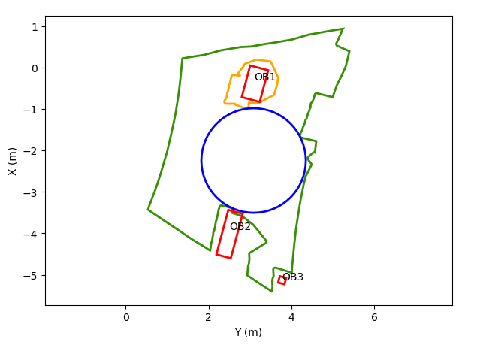
\includegraphics[width=0.99\textwidth]{chapter_6_experiments/imgs/experiments_1.pdf}
        \caption{}
        \label{fig:ch6_experiment_1}
    \end{subfigure}
    % \hfill
    \begin{subfigure}[t]{0.45\linewidth}
        \centering
        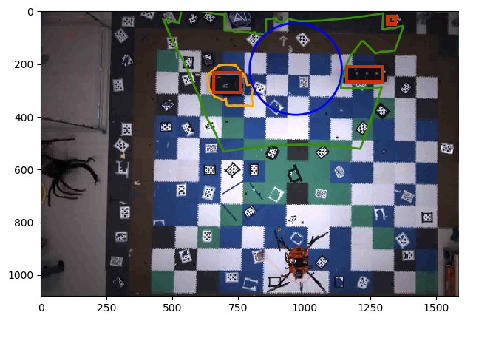
\includegraphics[width=0.99\textwidth]{chapter_6_experiments/imgs/experiments_2.pdf}
        \caption{}
        \label{fig:ch6_experiment_2}
    \end{subfigure}
    % \begin{subfigure}[t]{0.20\columnwidth}
    %     \centering
    %     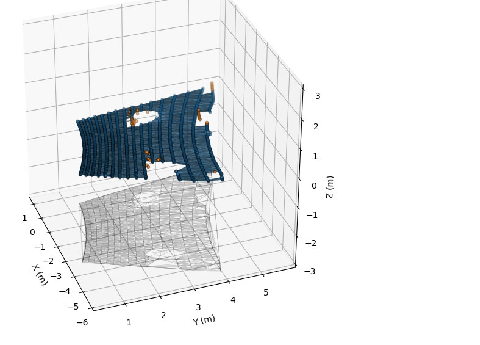
\includegraphics[trim=0cm 0cm 3cm 0cm, width=0.99\textwidth]{chapter_6_experiments/imgs/experiments_3.pdf}
    %     \caption{}
    %     \label{fig:ch6_experiment_3}
    % \end{subfigure}

    \caption{Landing site identification and selection from data collected at a NASA Langley facility. Obstacles positions are overlaid with red boxes. (a) Polylidar3D extracts a polygon of the surface represented as the the interior of the green polygon. The center of the blue circle is the selected touchdown point.  (b) Projection of all data onto an overhead camera.    }
    \label{fig:ch6_experiment}
    \hfill
\end{figure}

In real-time, every LiDAR scan was independently run through Polylidar3D and our selection algorithm.  In all cases the obstacles were captured accurately and a safe touchdown point was found. However there were cases ($\approx$ 5\%) where a stray LiDAR beam would cause a false positive causing non-optimal touchdown point selection. This motivated Polylidar3D refinment (already completed) to perform edge-preserving mesh smoothing and polygon filtering. Flight data captured at NASA Langley will be reprocessed with these updated Polylidar3D algorithms to guide future experiments.


\paragraph{Future Experiments}

Similar experiments will be performed in M-Air with different obstacle placements, sensor suites, lighting conditions, and potentially updates to Polylidar3D. We will primarily target use of a low-cost Intel RealSense L515 which is a \emph{solid state} LiDAR sensor. This device is significantly more lightweight (100 grams vs. 590+ grams) than a Velodyne unit and will offer a denser point cloud in the region of interest. We propose experiments where several elevated landing platforms will be placed in M-Air. Obstacles of varying size will be placed on these platforms. Different altitudes will tested, e.g., 3,6, and 9 meters above the ground.  Additionally instead of creating a mesh from a single scan,  multiple scans will be integrated to reduce noise using Truncated Signed Distance Function (TSDF) volume integration \cite{10.1145/237170.237269}. A final mesh will then be extracted with a marching cubes algorithm \cite{10.1145/37401.37422} and sent to Polylidar3D for flat surface extraction. 

\paragraph{Conclusion}

This chapter will extend offline landing site ID to an online (real-time) application supported by experimental validation.  Polylidar3D will extract flat surfaces from single scans and also from integrated meshes with multiple scans. A final journal publication will combine results from NASA and University of Michigan M-Air datasets.  We plan to submit results to the Journal of Field Robotics as well as a final dissertation chapter.






